%%%%hand and sets
\begin{frame}{}
    \begin{columns}
        \begin{column}{\textwidth}
            \centering
                \adjustbox{max width =\textwidth, min height=9cm}{%
                \begin{tikzpicture}
                    %hand
                    \visible<-7>{\node [above right,inner sep=0] (hand) at (0,0) {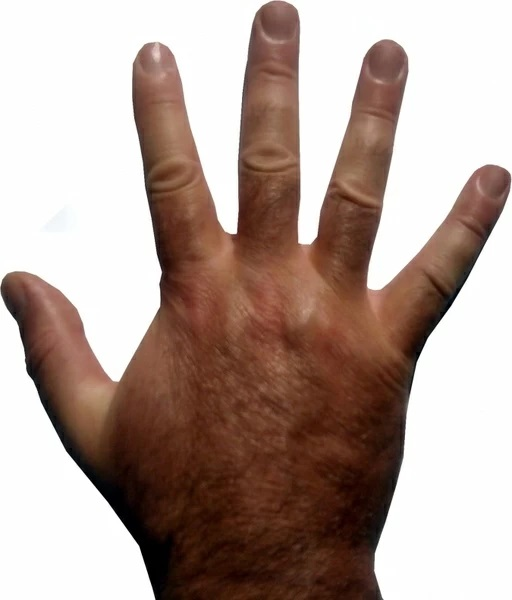
\includegraphics[width=3cm]{./images_5-20-2022/hand5.png}};}
                    
                    \node [above = .5cm of hand] (set) {{\visible<8->{\{}}\sun {\visible<8->{,}} \phone{\visible<8->{,}} \smiley{\visible<8->{,}} \twonotes{\visible<8->{,}} {\visible<7->{\frownie}}{\visible<8->{\}}} };
                          
                    \node<9-> [below = .5cm of set] (set2) {\{1, 2, 3, 4, 5\}};
                    % \draw[above right,help lines,step=5mm,gray!20] (0,0) grid (3,5);
                    
                    %thumb
                    \draw<2-7>[latex-, very thick, Green] (.5, 4.25) -- (.25, 1.95);
                    %index
                    \draw<3-7>[latex-, very thick, Green] (1.0, 4.25) -- (.9, 3.325);
                    %middle
                    \draw<4-7>[latex-, very thick, Green] (1.6, 4.25) -- (1.6125, 3.55);
                    %ring
                    \draw<5-7>[latex-, very thick, Green] (2.1, 4.25) -- (2.25, 3.325);
                    %pinky
                    \draw<6>[latex-, very thick, red] (2.58, 4.25) -- (2.85, 2.6) 
                    node[above, pos=0.1,red]{X};
                    \draw<7>[latex-, very thick, Green] (2.58, 4.25) -- (2.85, 2.6) ;
                    
                    %set arrows
                    \draw<9->[latex-, very thick, Green] (.5, 4.25) -- (.6, 3.45);
                    %index
                    \draw<9->[latex-, very thick, Green] (1.0, 4.25) -- (1.05, 3.45);
                    %middle
                    \draw<9->[latex-, very thick, Green] (1.6, 4.25) -- (1.5, 3.45);
                    %ring
                    \draw<9->[latex-, very thick, Green] (2.1, 4.25) -- (1.95, 3.45);
                    %pinky
                    \draw<9->[latex-, very thick, Green] (2.58, 4.25) -- (2.35, 3.45); 
                    
                    \node<10-> [below = .5cm of set2] (set3) {\{5, 4, 3, 5\}\textcolor{white}{, 1}};
                    
                    \draw<11->[-latex, very thick, Green] (.65, 3) -- (.65, 2.25);
                    %index
                    \draw<11->[-latex, very thick, Green] (1.05, 3) -- (1.05, 2.25);
                    %middle
                    \draw<11->[-latex, very thick, Green] (1.5, 3) -- (1.5, 2.25);
                    %ring
                    \draw<11->[-latex, very thick, Green] (1.95, 3) -- (1.95, 2.25);
                    %pinky
                    \draw<11->[-latex, very thick, red] (2.35, 3) -- (2.35, 2.25) node[below, pos=0.85,red]{X};
                    
                    \node<-7> [align =center ] at (-1.5,3) {More fingers \\or symbols?};
                    \node<12-> [below = .1cm of set3, align = center] {\tiny "The essence of math is not to make simple things complicated,\\ \tiny but to make \textit{complicated things simple}."};
                \end{tikzpicture}
                }
        \end{column}
    \end{columns}
\end{frame}

%%%hilbert hotel%%%
\begin{frame}{}
    % \Large \textbf{What is Math(s)?}
    % \normal
    % \null \vfill
    \colorlet{soulred}{red!25}
    \colorlet{soulgreen}{green!25}
    \begin{columns}
        \begin{column}{.43\textwidth}
             \uncover<3->{\textbf{Are these two sets the same?}} 
             \\ \uncover<4->{\hspace{.5cm} No.} 
             \\ \uncover<5->{\textbf{Are these two sets the same \textit{size}?}}
             \\ \uncover<16->{\hspace{.5cm} Yes!}
             \begin{itemize}
                 \item<2->[]\sethlcolor{soulred}\hl<2>{$\mathbb{N} = \{1, 2, 3, 4, \dots\}$}
                 \item<3->[]\sethlcolor{soulgreen}\hl<3>{$\mathbb{N}_{0} = \{0, 1, 2, 3, 4, \dots\}$} 
             \end{itemize}
                %%%%%%venn diagram
                \vspace{6pt}
                \begin{tikzpicture}[scale=1.0, envel/.style={shape=ellipse, draw, inner sep=-0.5cm}]
                	\def\circleA{(1.4,0) circle (1)} 
                	%\node[anchor=south] at (current bounding box.north) {$A \cap B$}; 
                    \large
                    \node (1) at (1.5,.5) {$1$};
                    \node (2) at (1.65,-.5) {$2$};
                    \node (3) at (1.25,.75) {$3$};
                    \node (4) at (.6,-.1) {$4$};
                    \node (0) at (0,0) {$0$};
                    \node (-5) at (-1.5,.65) {$-5$};
                    \node (sqrt) at (3.25,.25) {$\sqrt{2}$};
                    \node (pi) at (3.5,-1) {$\pi$};
                    \node (frac1) at (-1.6,-1.125) {$-\frac{1}{2}$};
                    \node (frac2) at (2.8,1) {$\frac{5}{3}$};
                	\node<3->[draw, thick, fill = green!35, inner sep=.15cm, fit=(1)(2)(3)(0),shape=ellipse] (gc) { };
                	\draw<2->[draw, thick, fill = red!35] \circleA node {\dots }; 
                    \foreach \n in {0,1,2,3,4} {%
            	        \node at (\n) {$\n$};
                	}   
                    % \node (a) at (1.25,4.25) {$2$};
                	\draw[very thick] (-2,-2) rectangle (4,2) node[anchor=north west] at (current bounding box.north west) {$\mathbb{R}$}; 
                \end{tikzpicture}
                %%%%%%%%%%%%
        \end{column}
        \only<6->{%
        \begin{column}{.5\textwidth}
            \textbf{The Hilbert Hotel Problem}
            % \vspace{12pt}
            \only<7>{%
                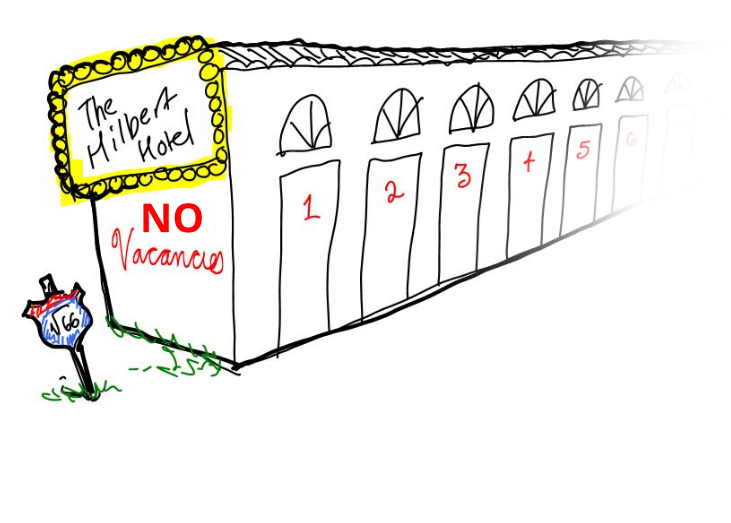
\includegraphics[width =\textwidth]{./images_5-20-2022/hilbert_hotel0.png}
            }
            \only<8>{%
                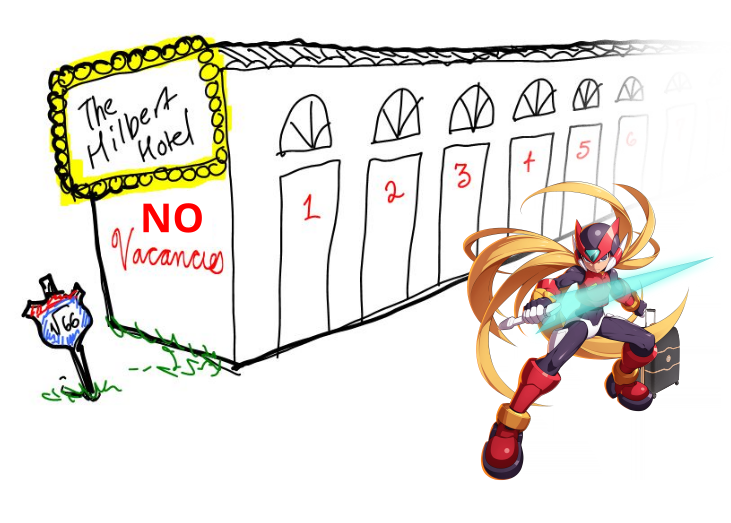
\includegraphics[width =\textwidth]{./images_5-20-2022/hilbert_hotel1.png}
                }
            \only<9>{%
                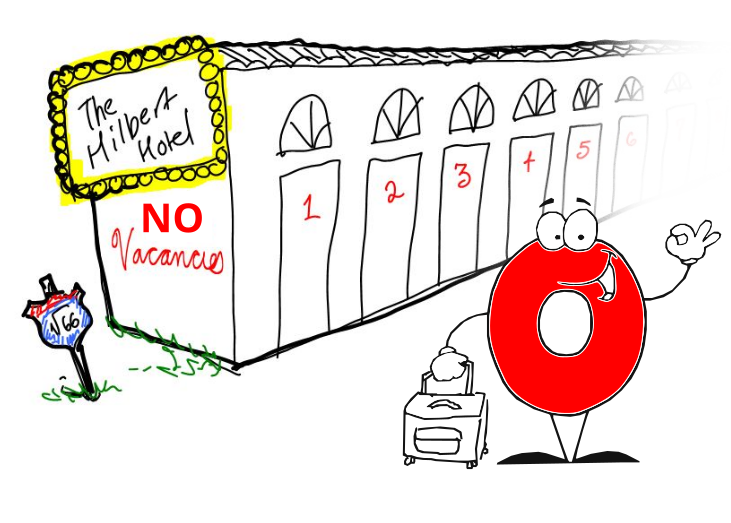
\includegraphics[width =\textwidth]{./images_5-20-2022/hilbert_hotel2.png}
            }
            \only<10>{%
            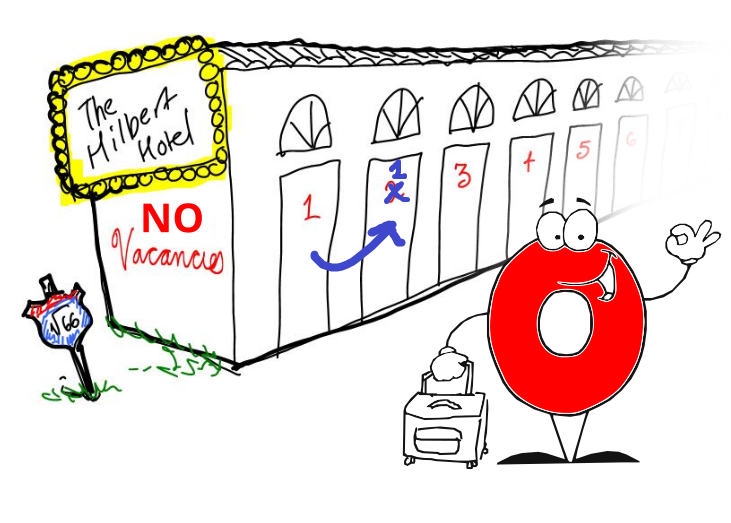
\includegraphics[width =\textwidth]{./images_5-20-2022/hilbert_hotel3.png}}
            \only<11>{%
            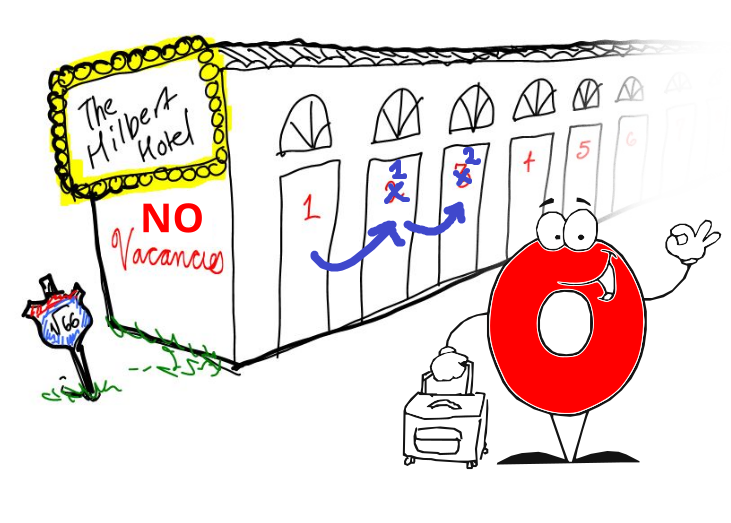
\includegraphics[width =\textwidth]{./images_5-20-2022/hilbert_hotel4.png}}
            \only<12>{%
            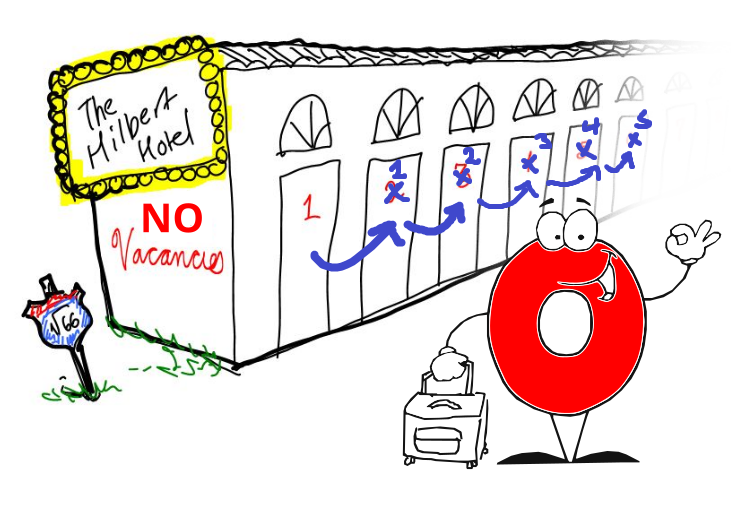
\includegraphics[width =\textwidth]{./images_5-20-2022/hilbert_hotel5.png}}
            \only<13>{%
            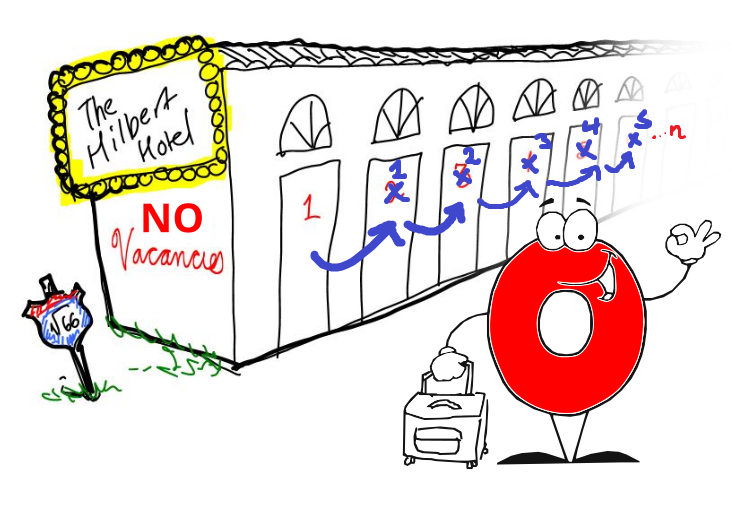
\includegraphics[width =\textwidth]{./images_5-20-2022/hilbert_hotel6.png}}
            \only<14>{%
            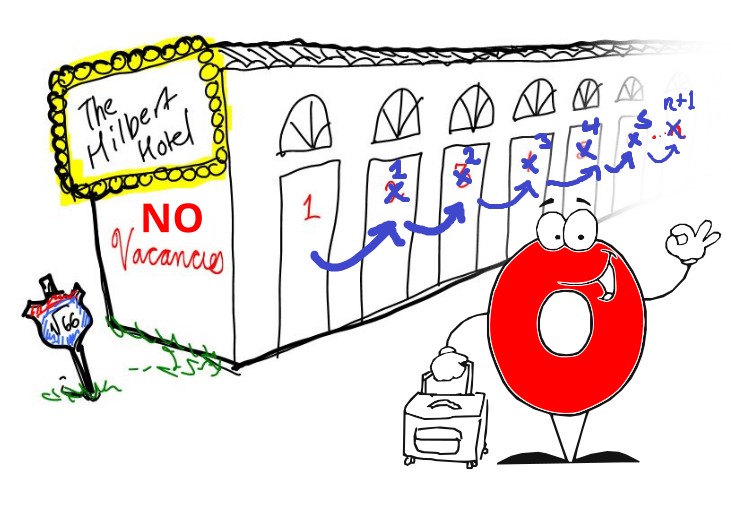
\includegraphics[width =\textwidth]{./images_5-20-2022/hilbert_hotel7.png}}
            \only<15->{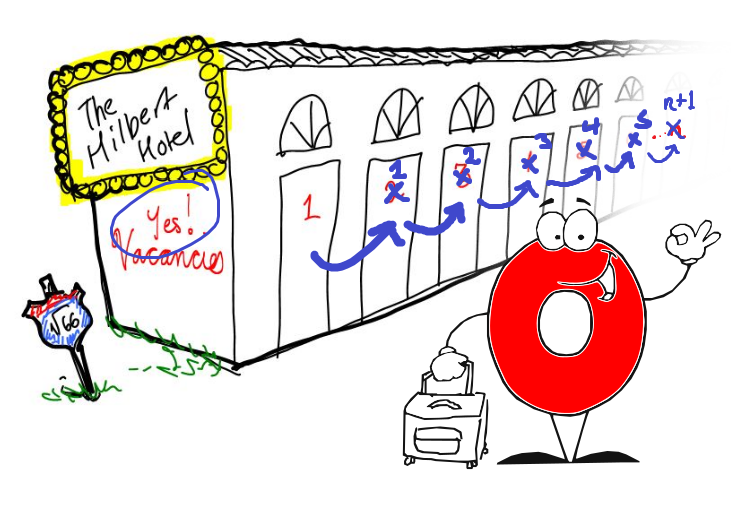
\includegraphics[width =\textwidth]{./images_5-20-2022/hilbert_hotel8.png}}
            \\ \only<17->{We call these sets \textit{countable}} 
            \only<18->{\dots because we can \textit{count} them.}
        \end{column}
        }
    \end{columns}
    % \vfill
\end{frame}

% rational numbers countable
\begin{frame}{}
    \begin{columns}
        \colorlet{soulblue}{blue!25}
        \colorlet{soulred}{red!25}
        \begin{column}{.43\textwidth}
             \textbf{Are these two sets the same size?}
             \\ \uncover<33->{\hspace{.5cm} Yes!}
             \begin{itemize}
                 \item<1->[]\sethlcolor{soulred}\hl<1>{$\mathbb{N} = \{1, 2, 3, 4, \dots\}$}
                 \item<2->[]\sethlcolor{soulblue}\hl<2>{$\mathbb{Q} = \{\frac{1}{2}, \frac{3}{4}, \frac{5}{3}, -1, 4, 0,\dots\}$} 
             \end{itemize}
                %%%%%%venn diagram
                \vspace{6pt}
                \begin{tikzpicture}[scale=1.0, envel/.style={shape=ellipse, draw, inner sep=-0.5cm}]
                	\def\circleA{(1.4,0) circle (1)} 
                    \large
                	%nodes must be defined previously
                	\node<2->[draw,fill = blue!25, inner sep=.5ex, rounded corners =.7cm, thick, fit=(frac1) (frac2)] { };
                	\draw[draw, thick, fill = red!35] \circleA node {\dots }; 
                	
                    \node (1) at (1.5,.5) {$1$};
                    \node (2) at (1.65,-.5) {$2$};
                    \node (3) at (1.25,.75) {$3$};
                    \node (4) at (.6,-.1) {$4$};
                    \node (0) at (0,0) {$0$};
                    \node (-5) at (-1.5,.65) {$-5$};
                    \node (sqrt) at (3.25,.25) {$\sqrt{2}$};
                    \node (pi) at (3.5,-1) {$\pi$};
                    \node (frac1) at (-1.6,-1.125) {$-\frac{1}{2}$};
                    \node (frac2) at (2.8,1) {$\frac{5}{3}$};
                	\draw[very thick] (-2.25,-2) rectangle (4,2) node[anchor=north west] at (current bounding box.north west) {$\mathbb{R}$}; 
                \end{tikzpicture}
                \centering
                \vspace{-10pt}
                
                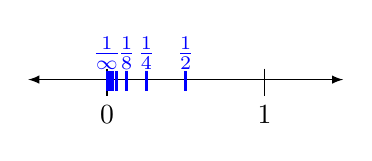
\begin{tikzpicture}[scale=2.0]
                    \node<3->[above,white] at (.5,0) {$\frac{1}{2}$};
                    \draw<3->[latex-latex] (-.5,0) -- (1.5,0) ; %edit here for the axis
                	\foreach \x in  {0,1} 
                        \draw<3->[shift={(\x,0)},color=black] (0pt,2pt) -- (0pt,-2pt);
                	\foreach \x in  {0,1} 
                        \draw<3->[shift={(\x,0)},color=black] (0pt,0pt) -- (0pt,-3pt) node[below] {$\x$};
                    \node<4->[above,blue] at (.5,0) {$\frac{1}{2}$};
                        \draw<4->[blue,color=blue,very thick] (.5,1.5pt) -- (.5,-2pt);
                    \node<5->[above,blue] at (.25,0) {$\frac{1}{4}$};
                        \draw<5->[blue,color=blue,very thick] (.25,1.5pt) -- (.25,-2pt);
                    \node<6->[above,blue] at (.125,0) {$\frac{1}{8}$};
                        \draw<6->[blue,color=blue,very thick] (.125,1.5pt) -- (.125,-2pt);
                    \foreach \x in {16,32,64,128,256}
                        \draw<7->[blue,color=blue,very thick] ({1/\x},1.5pt) -- ({1/\x},-2pt);
                    \node<8->[above,blue] at (0.0001,0) {$\frac{1}{\infty}$};
                \end{tikzpicture}
                
                %%%%%%%%%%%%
        \end{column}
        %%%%%
        \only<9->{%
        \begin{column}{.5\textwidth}
            \vspace{15pt}
            \only<10>{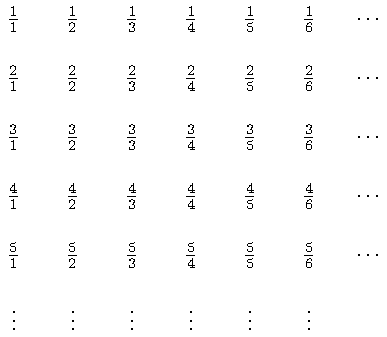
\includegraphics[width =\textwidth]{./images_5-20-2022/rationalmaps_9.pdf}}
            \only<11>{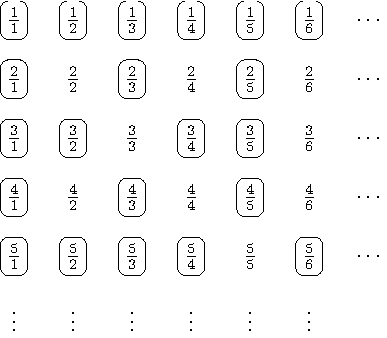
\includegraphics[width =\textwidth]{./images_5-20-2022/rationalmaps_11.pdf}}
            \only<12>{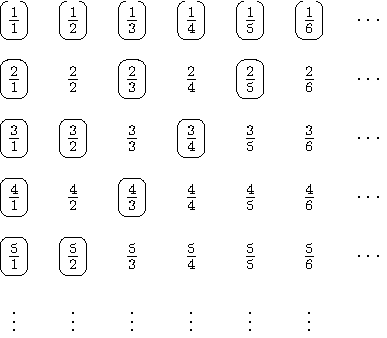
\includegraphics[width =\textwidth]{./images_5-20-2022/rationalmaps_14.pdf}}
            \only<13>{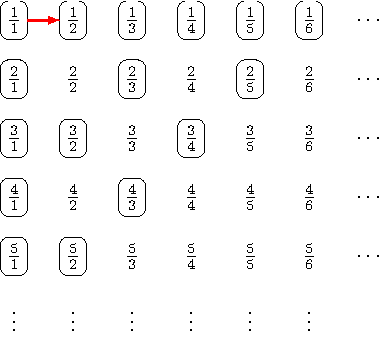
\includegraphics[width =\textwidth]{./images_5-20-2022/rationalmaps_17.pdf}}
            \only<14>{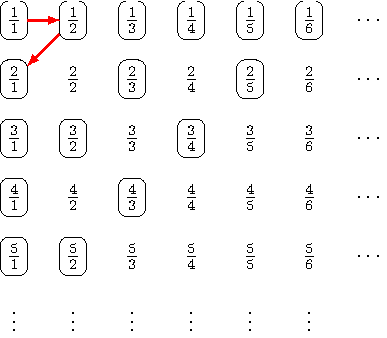
\includegraphics[width =\textwidth]{./images_5-20-2022/rationalmaps_4.pdf}}
            \only<15>{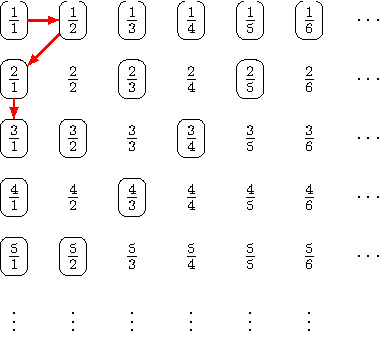
\includegraphics[width =\textwidth]{./images_5-20-2022/rationalmaps_5.pdf}}
            \only<16>{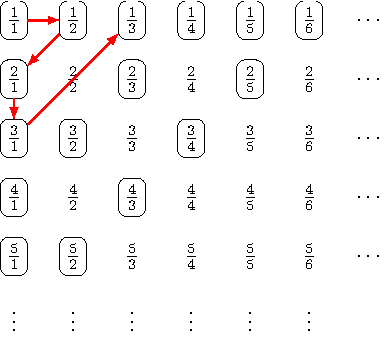
\includegraphics[width =\textwidth]{./images_5-20-2022/rationalmaps_15.pdf}}
            \only<17>{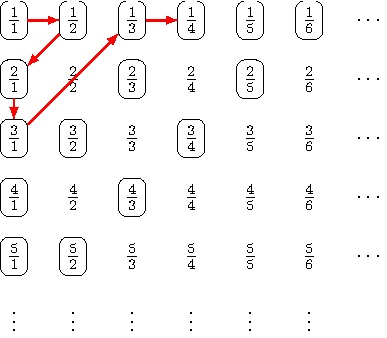
\includegraphics[width =\textwidth]{./images_5-20-2022/rationalmaps_18.pdf}}
            \only<18>{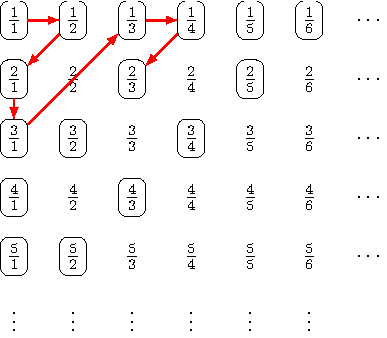
\includegraphics[width =\textwidth]{./images_5-20-2022/rationalmaps_3.pdf}}
            \only<19>{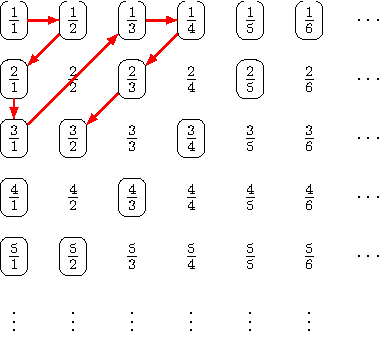
\includegraphics[width =\textwidth]{./images_5-20-2022/rationalmaps_16.pdf}}
            \only<20>{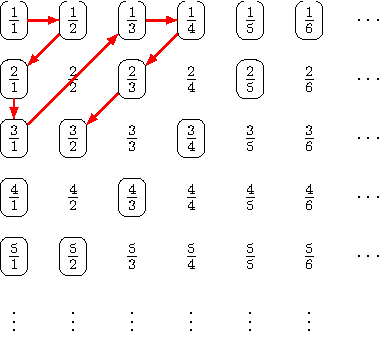
\includegraphics[width =\textwidth]{./images_5-20-2022/rationalmaps_19.pdf}}
            \only<21>{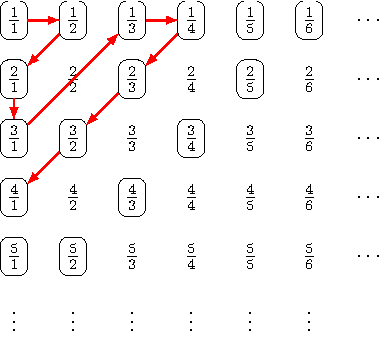
\includegraphics[width =\textwidth]{./images_5-20-2022/rationalmaps_20.pdf}}
            \only<22>{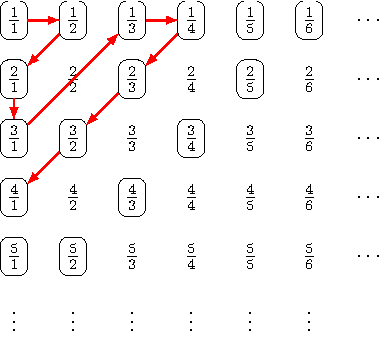
\includegraphics[width =\textwidth]{./images_5-20-2022/rationalmaps_1.pdf}}
            \only<23>{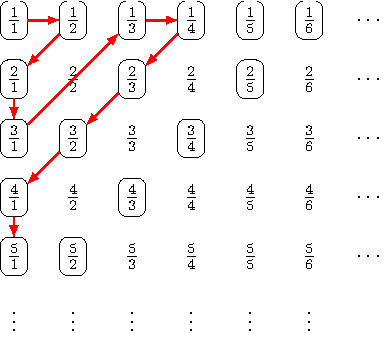
\includegraphics[width =\textwidth]{./images_5-20-2022/rationalmaps_2.pdf}}
            \only<24>{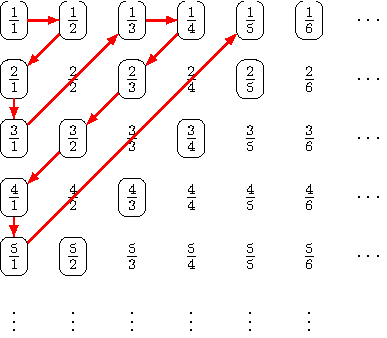
\includegraphics[width =\textwidth]{./images_5-20-2022/rationalmaps_0.pdf}}
            \only<25>{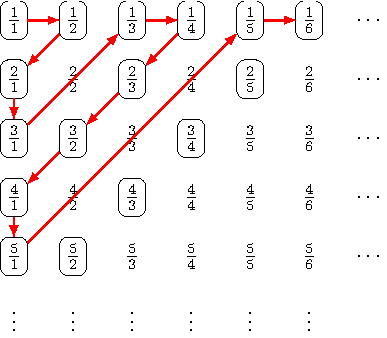
\includegraphics[width =\textwidth]{./images_5-20-2022/rationalmaps_6.pdf}}
            \only<26>{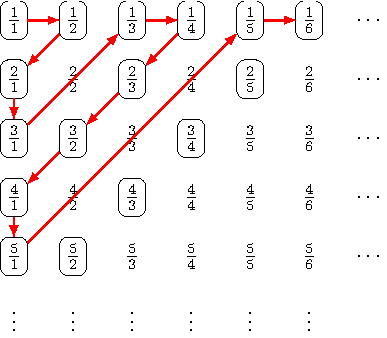
\includegraphics[width =\textwidth]{./images_5-20-2022/rationalmaps_7.pdf}}
            \only<27>{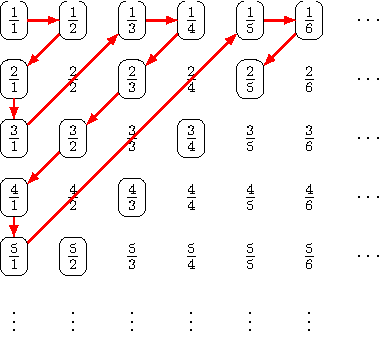
\includegraphics[width =\textwidth]{./images_5-20-2022/rationalmaps_8.pdf}}
            \only<28>{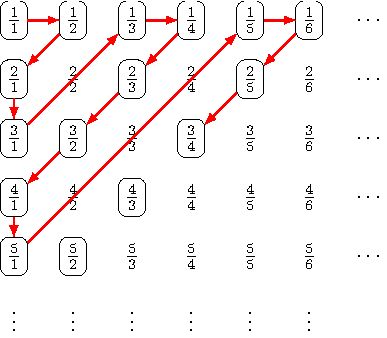
\includegraphics[width =\textwidth]{./images_5-20-2022/rationalmaps_10.pdf}}
            \only<29>{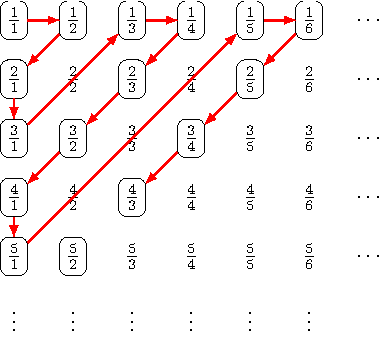
\includegraphics[width =\textwidth]{./images_5-20-2022/rationalmaps_12.pdf}}
            \only<30>{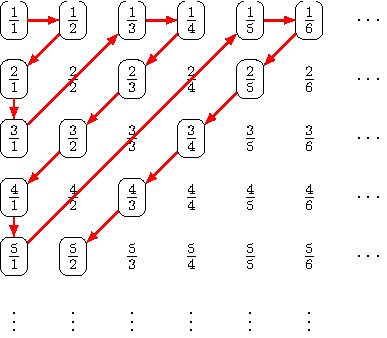
\includegraphics[width =\textwidth]{./images_5-20-2022/rationalmaps_13.pdf}}
            \only<31->{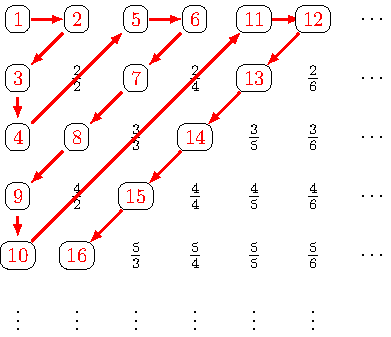
\includegraphics[width =\textwidth]{./images_5-20-2022/rationalmaps_21.pdf}}
            
        \end{column}
        }
    \end{columns}
    % \vfill
\end{frame}

\begin{frame}
    \centering
    \Large
    \vfill
    These are example of "direct" proofs.
    \vfill
\end{frame}


\begin{frame}{}
    \begin{columns}
        \begin{column}{.5\textwidth}
        \textbf{Are all infinite sets the same size?}
        \\\Large 
        \only<2-3>{$|\infty| = |\infty|$?} 
        \only<4-30>{$|\{1, 2, 3, 4, \dots \}| = |\mathbb{R}|$?}
        % \only<12-30>{$|\{1, 2, 3, 4, \dots \}| =$ \normalsize$|\{x\in \mathbb{R}| 0<x<4\}|$?}
        % \normalsize
        \only<31->{No -different infinities!}
            \only<3->{%
                \begin{figure}
                    \centering
                    \includegraphics<3-30>[width =.5\textwidth]{./images_5-20-2022/Georg_Cantor.png}
                    \includegraphics<31>[width =.5\textwidth]{./images_5-20-2022/Georg_Cantor_eyes.png}
                    \includegraphics<32>[width =.5\textwidth]{./images_5-20-2022/Georg_Cantor_eyes_smile.png}
                    \includegraphics<33>[width =.5\textwidth]{./images_5-20-2022/Georg_Cantor_eyes_sad.png}
                    \only<3->{\caption*{Georg Cantor (1845-1918)}}
                    % \icncludegraphics<34>[width =\textwidth]{./images_women_in_IT/HannahCairo-cr.ValeriePlesch-Screen-scaled.png}
                    % \only<34>{\caption*{Mizohata-Takeuchi conjecture\\ Hannah Cairo (2008--)}}
                \end{figure}
                }
        \end{column}
        %%%%
        \begin{column}{.5\textwidth}
            \uncover<5-10>{\textbf{What are the \textit{Real} numbers ($\mathbb{R}$)?}}
            \vspace{10pt}
            
            \only<5-12>{%
                \begin{tikzpicture}[scale=.85]
                    \draw[white] (0,1) circle (1); 
                    \draw[latex-latex] (-1.75,0) -- (5.75,0) ; %edit here for the axis
                        \foreach \x in  {-1,0,1,2,3,4,5} 
                            \draw[shift={(\x,0)},color=black] (0pt,2pt) -- (0pt,-2pt);
                        \foreach \x in {-1,0,1,2,3,4,5} 
                            \draw[shift={(\x,0)},color=black] (0pt,0pt) -- (0pt,-3pt) node[below] {$\x$};
                    \draw<6>[blue, very thick,*-*,text = blue] (0,0) -- (2.5,0) node[above = 3pt] {2.5};
                    \draw<7>[blue, very thick,*-*,text = blue] (0,0) -- (4.25,0) node[above = 3pt] {4.25};
                    \draw<8>[blue, very thick,*-*,text = blue] (0,0) -- (1.41421,0) node[above = 3pt] {$\sqrt{2}$};
                    \draw<9> (0,1) circle (1); 
                    \draw<9>[dashed,*->] (0,1)--(-1,1) node[pos=.5,above] {1}; 
                    \draw<9>[blue, very thick, *-*] (0,0) arc (-90:90:1) node[pos=.5, right] {$\pi \approx 3.14\dots$};
                    \draw<10> (3.1416,1) circle (1);
                    \draw<10>[blue, very thick,*-*,text = blue] (0,0) -- (3.1416,0) node[above = 3pt] {$\pi \approx 3.14\dots$};
                    \draw<11-12>[blue, very thick,o-o] (0,0) -- (4,0) node[above, pos=.5] {$(0,4)\subseteq \mathbb{R}$};
                \end{tikzpicture}
            }
            \only<13-33>{%
                \textit{Assume} this set is \textit{countable}, then you could write out a list, like this:\\
                \large \centering
                \vspace{20pt}
                \setlength\tabcolsep{1pt} % default value: 6pt
                \begin{tabular}{cccccccc}
                    \uncover<14->{1 & \textbf{$\rightarrow$} & 3.\only<19-20,29->{\cellcolor{green}} & 1 & 4 & 1 & 5 & \dots\\}
                    \uncover<15->{2 & \textbf{$\rightarrow$} & 2. & 5 \only<21-22,29->{\cellcolor{green}}& 0 & 0 & 0 & \dots\\}
                    \uncover<16->{3 & \textbf{$\rightarrow$} & 0. & 1 & 2\only<23-24,29->{\cellcolor{green}} & 5 & 0 & \dots\\}
                    \uncover<17->{4 & \textbf{$\rightarrow$} & 3. & 9 & 9 & 9\only<25-26,29->{\cellcolor{green}} & 9 & \dots\\}
                    \uncover<17->{5 & \textbf{$\rightarrow$} & 1. & 2 & 3 & 4 & 5\only<27-28,29->{\cellcolor{green}} & \dots\\}
                    \uncover<17->{\vdots & \vdots & \vdots & \vdots & \vdots & \vdots & \vdots & \\}
                \end{tabular}
                
                \begin{tabular}{cccccccc}
                     \uncover<18->{$d$} \cellcolor{white} & \uncover<20->{= \cellcolor{white} & 2.} \only<30->{\cellcolor{red!25}}& \uncover<22->{4} \only<30->{\cellcolor{red!25}}& \uncover<24->{1} \only<30->{\cellcolor{red!25}}& \uncover<26->{8} \only<30->{\cellcolor{red!25}}& \uncover<28->{4} \only<30->{\cellcolor{red!25}}& \uncover<30->{\dots}\only<30->{\cellcolor{red!25}}\\
                \end{tabular}
            }
        \end{column}
    \end{columns}
\end{frame}

\begin{frame}
    \Large
    \centering
    Proof by \textit{contradiction}
    \vspace{10pt}
    \normalsize

    \only<2>{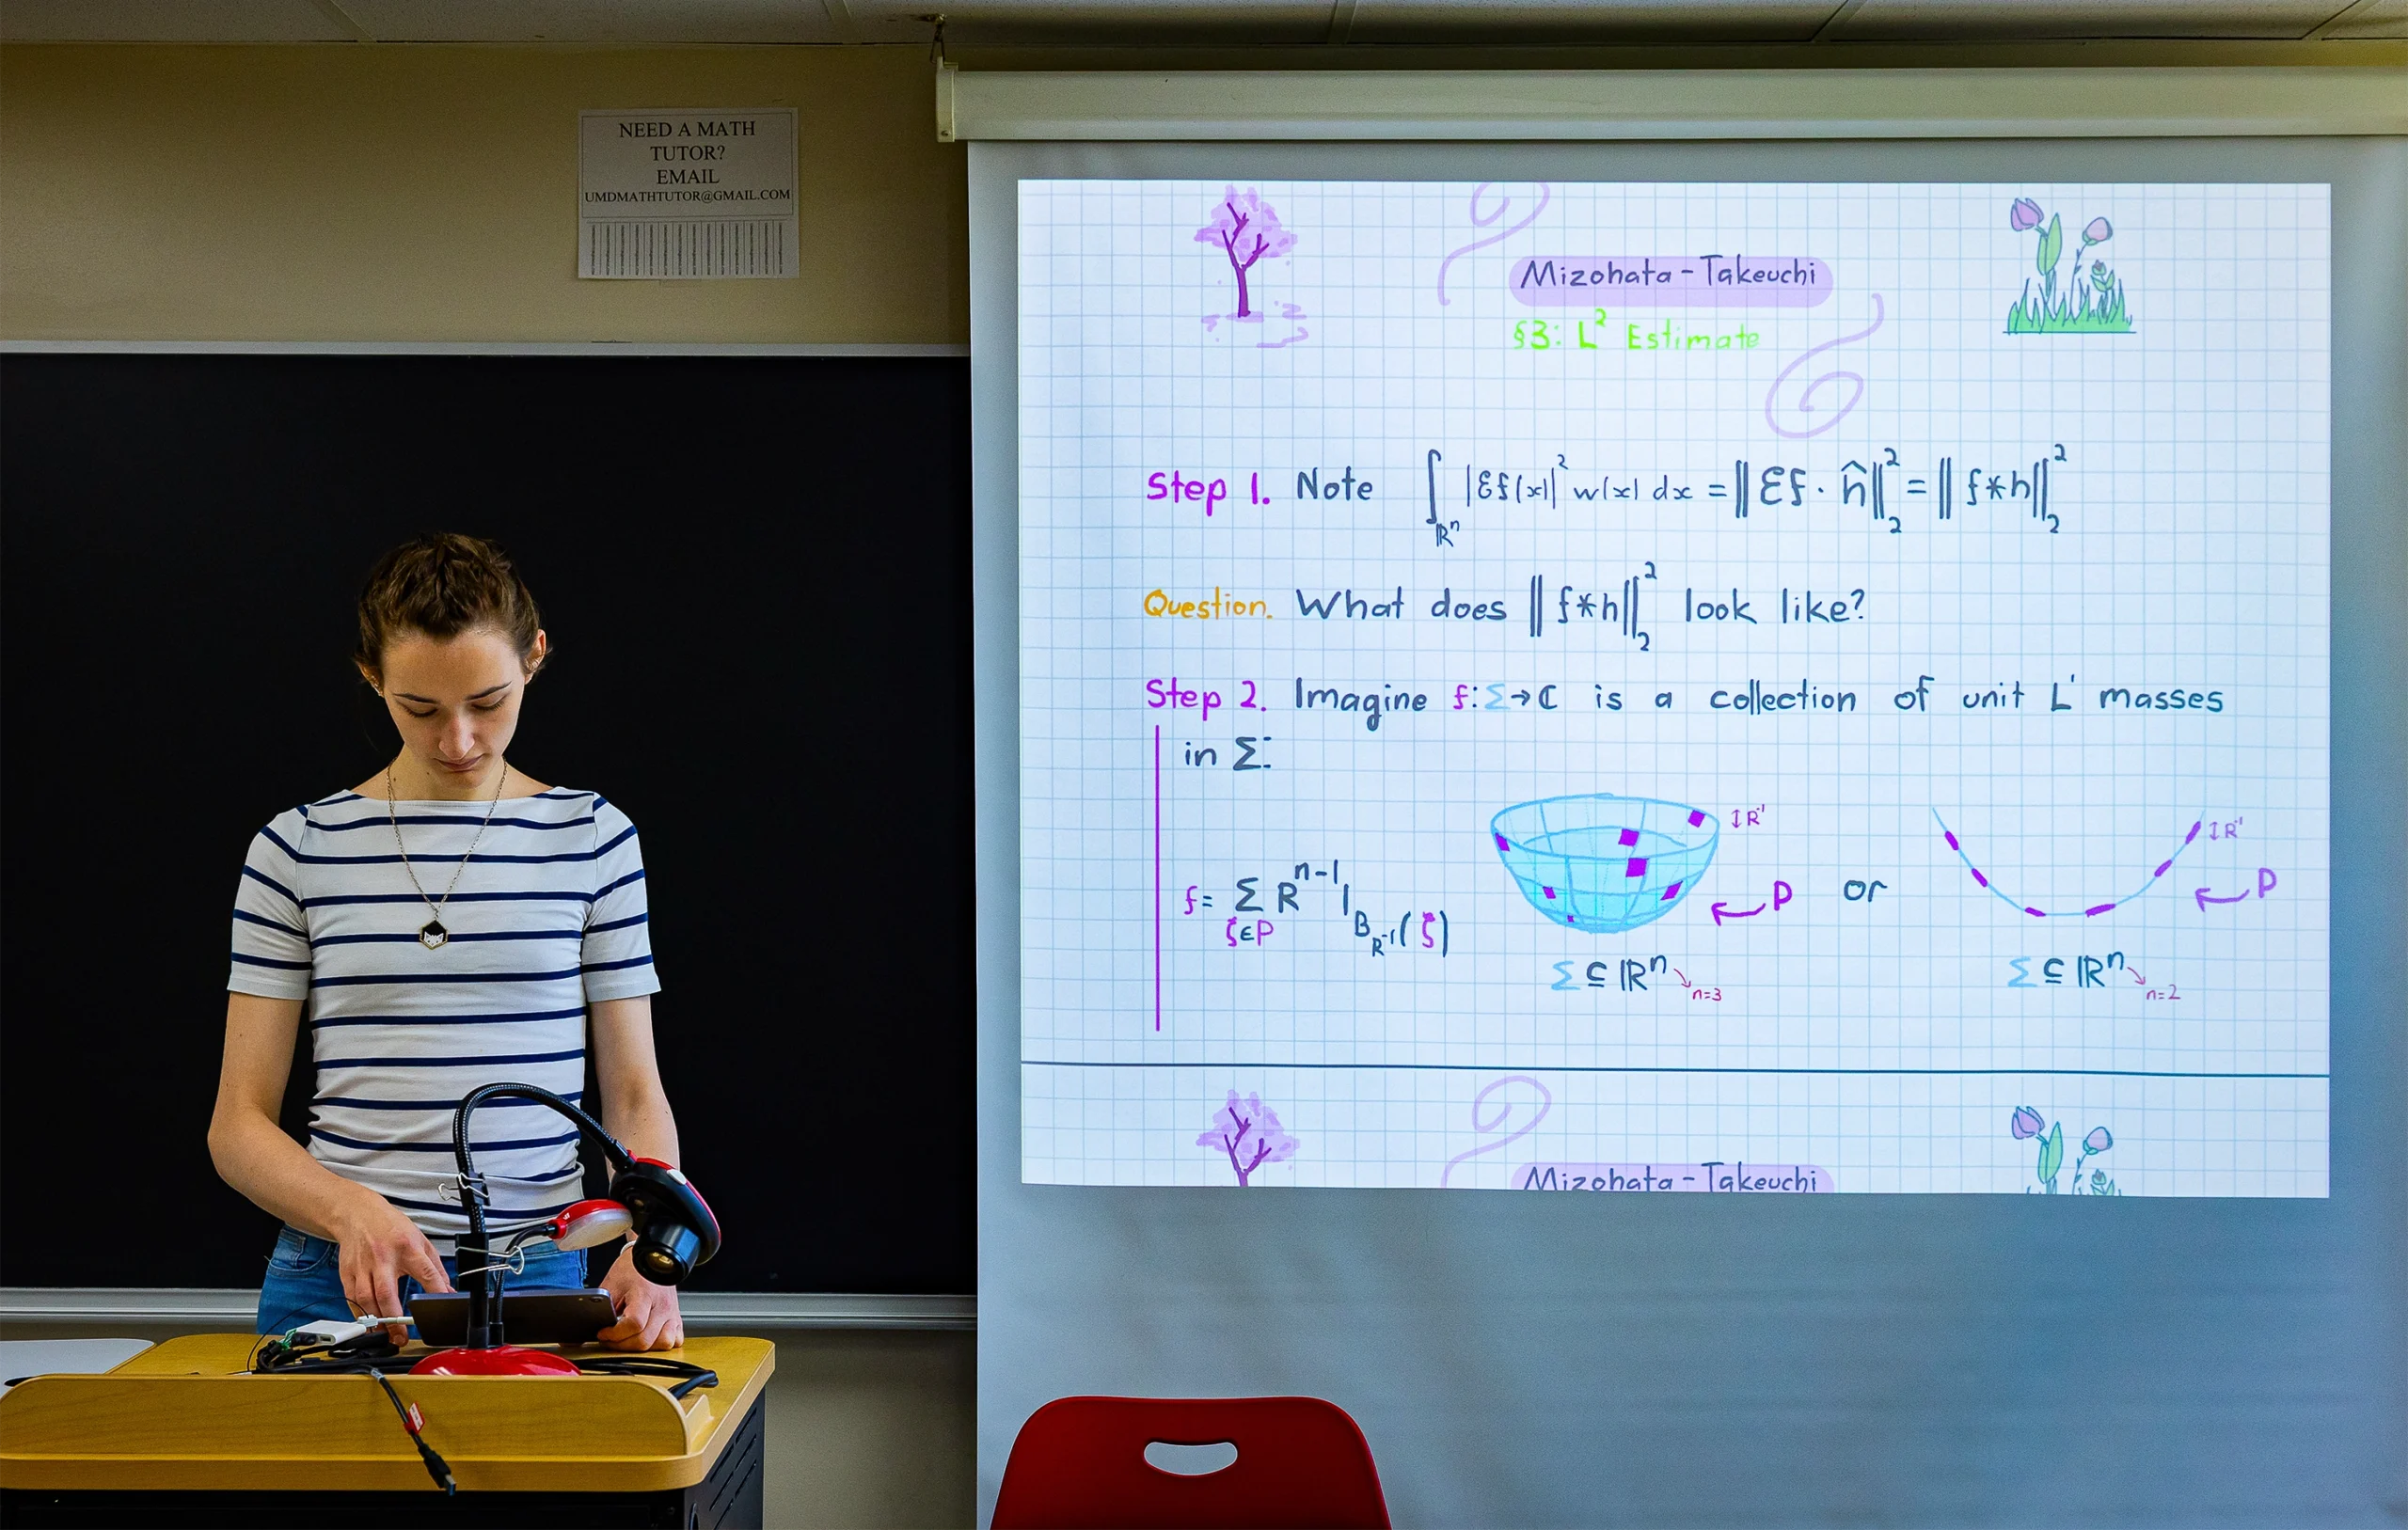
\includegraphics[width =.6\textwidth]{./images_women_in_IT/HannahCairo-cr.ValeriePlesch-Screen-scaled.png} \\
        Mizohata-Takeuchi conjecture\\ Hannah Cairo    
    }
    \only<3>{\includegraphics<3->[width =.6\textwidth]{./images_women_in_IT/Summer_Haag_Clyde_Kertzer.png}\\
            local-global conjecture\\ Summer Haag and Clyde Kertzer
    }
    % \begin{columns}
    %     \begin{column}{.45\textwidth}
    %         % Mizohata-Takeuchi conjecture\\ Hannah Cairo (2008--)
    %     \end{column}
    %     \begin{column}{4.5\textwidth}
    %     \end{column}
    % \end{columns}
\end{frame}

%%Boolean%%%%%%
%%pyramid%%%
\begin{frame}{}
    \begin{columns}
        \begin{column}{.5\textwidth}
        \textbf{\null}%place holder
        \\ \centering \huge 
        \normalsize
            \only<2->{\begin{figure}
                \centering
                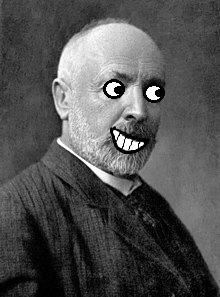
\includegraphics[width =.6\textwidth]{./images_5-20-2022/Georg_Cantor_eyes_smile.png}
                \caption*{Georg Cantor (1845-1918)}
            \end{figure}}
            % \only<5->{\begin{figure}
            %     \centering
            %     \vspace{20pt}
            %     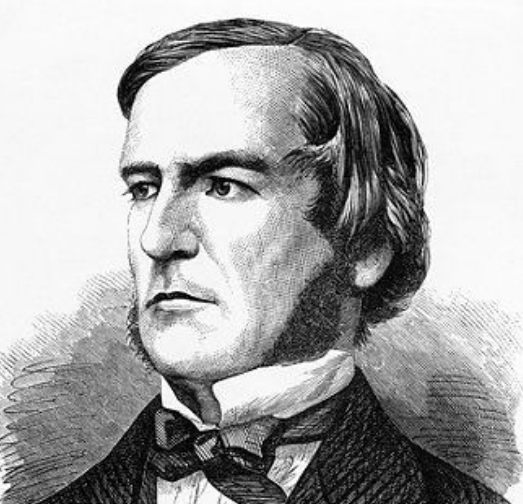
\includegraphics[width =.6\textwidth]{./images_5-20-2022/Boole.png}
            %     \caption*{George Boole (1815-1864)}
            % \end{figure}}
        \end{column}
        %%%%
        \begin{column}{.5\textwidth}
            \vspace{10pt}
            \begin{figure}
                \includegraphics<1>[width=.8\textwidth]{./images_5-20-2022/mathpyramid1.png}
                \includegraphics<2>[width=.8\textwidth]{./images_5-20-2022/mathpyramid2.png}
                % \includegraphics<3>[width=.8\textwidth]{./images_5-20-2022/mathpyramid3.png}
                % \includegraphics<4->[width=.8\textwidth]{./images_5-20-2022/mathpyramid4.png}
            \end{figure}
            
        \end{column}
    \end{columns}
\end{frame}
